\documentclass[../poliXuniversity_hospital_(USP)_report.tex]{subfiles}

\begin{document}
Um grupo de extensão é um cojunto de alunos que se reunem para realização de alguma atividade. Esses grupos são independentes e as todas as atividades são realizadas por alunos. Responsabilidades financeiras, fiscais, captação de recursos, treinamento dos membros e manutenção do espaço físico são responsabilidades do equipe a qual possui um professor orientador para suporte docente. Na Escola Politécnica existem diversos grupos de extensão, alguns focados em competições, outros em prestação de serviço, pesquisa e ensino. A ZIMA surgiu da vontade de perpetuar o conhecimento e o impacto da tecnologia na saúde dentro da comunidade USP.

\begin{figure}[h]
\centering
    \caption{Logo ZIMA}
    \centering % para centralizarmos a figura
    
\includegraphics[width=14cm]{images/logo_zima.png}
    \caption*{Fonte: Autor}
    \label{figura: Logo ZIMA}
\end{figure}
\chapter{Porque zima?}
As enzimas são responsáveis por catalisar reações, garantindo eficiência e melhor funcionamento da célula. Analogamente, dentro de um hospital, nossa tecnologia exerce uma função similar, otimizando processos e garantindo que o atendimento ao paciente seja feito com maior velocidade e segurança. É através dessa analogia que surgiu o nome ZIMA, abreviação de "enzima". Somos um grupo de extensão da POLI cuja missão, ao construir cada um de nossos projetos, é melhorar a qualidade dos processos hospitalares, garantindo que esse ambiente seja construído de forma mais confortável e ao mesmo tempo eficiente.


\chapter{Nossos Pilares}
\section{Conhecimento em livre acesso}
A ZIMA tem como pilar a produção de conhecimento livre, em "Open Source", de modo que nossa pesquisa seja acessível e replicável por qualquer instituição que tenha como objetivo a aplicação de tecnologia hospitalar com a finalidade de trazer melhor qualidade de tratamento para pacientes independente de onde, quando e por quem. 

\section{Aprendizado e experiência}
Em meio a projetos, fabricações e testes, priorizamos desenvolver e evoluir cada integrante do time. Nossa responsabilidade não se limita a entregar os projetos ao hospital, mas formar engenheiros mais capacitados. E não apenas em habilidades técnicas mas também com a vivencia do ambiente hospitalar, para que no futuro encarem desafios ainda maiores e que impactem a sociedade através da inovação

\section{Soluções viáveis}
Sabemos que a única maneira de expandir nosso impacto é com uma tecnologia de custo acessível e um equipamento de produção escalável. Portanto, nos comprometemos a criar soluções que sejam implementáveis tanto no ponto de vista econômico quanto industrial tornando a solução aplicável no setor público e privado.


\chapter{Estrutura}
O grupo é divido em uma capitania, coordenadores de área e membros de área. Cada um com suas determinadas funções.
\begin{figure}[h!]
\centering
    \caption{Estrutura ZIMA}
    \centering % para centralizarmos a figura
    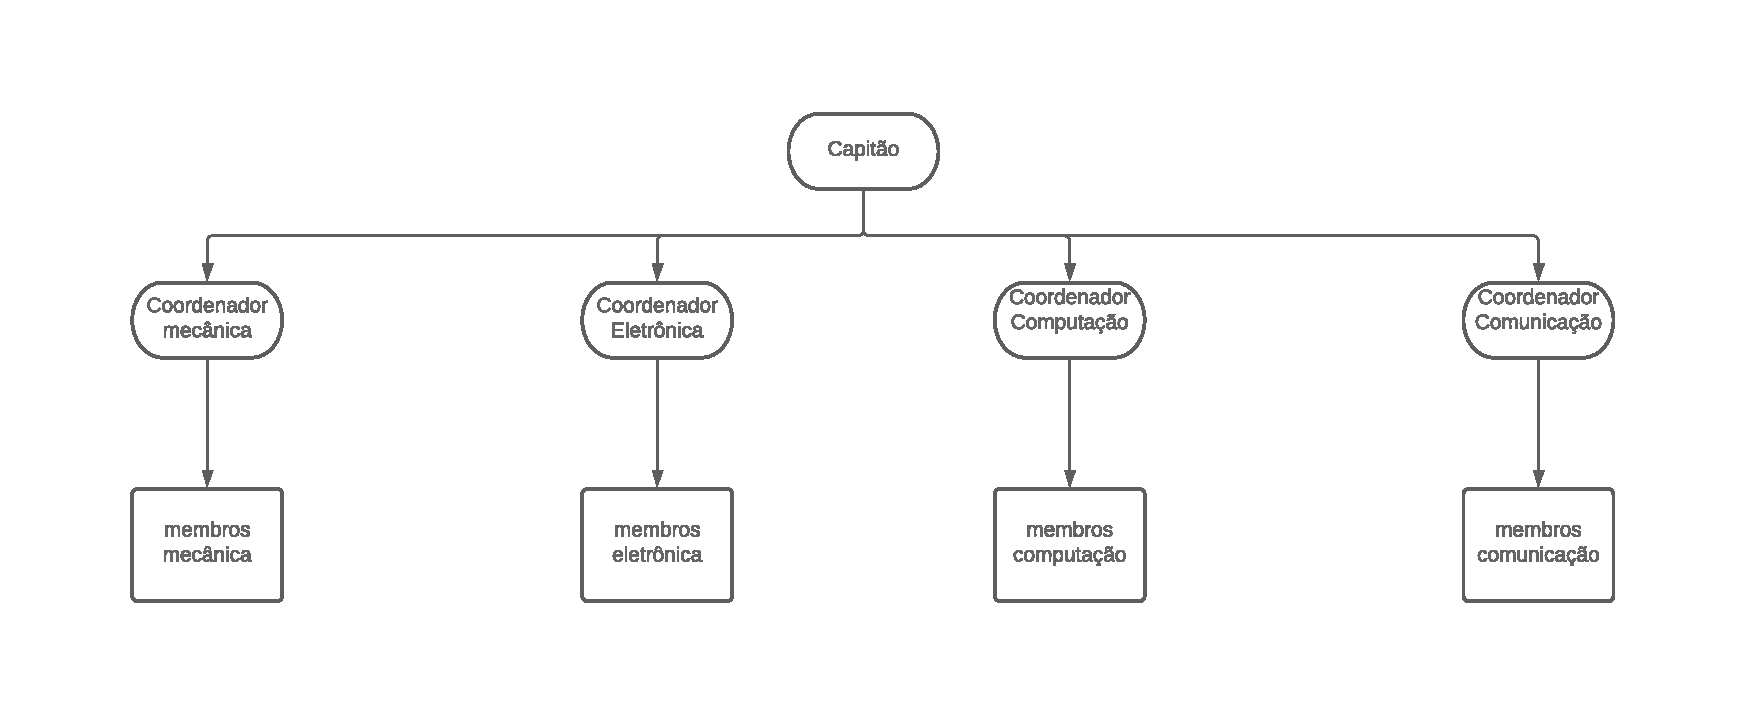
\includegraphics[width=17cm]{images/diagrama_zima.pdf}
    \caption*{Fonte: Autor}
    \label{figura: Estrutura ZIMA}
\end{figure}

ATRIBUIÇÕES COORDENAÇÃO MECÂNICA:

A coordenação é responsável por gerir os projetos da área, tendo como responsabilidade realizar a gestão de pessoas na área, garantir a realização das tarefas, certificar a qualidade dos projetos desenvolvidos e dar suportes aos membros no que se diz a respeito de realização de tarefas e dúvidas no desenvolvimento do projeto.

ATRIBUIÇÕES COORDENAÇÃO COMUNICAÇÃO:

A coordenação da comunicação é responsável por realizar a gestão da área, tendo como principais atribuições a garantia de realização de tarefas, o desenvolvimento de maneiras de captação de recursos, a contribuição na realização de tarefas, a certificação da qualidade das atividades desenvolvidas. Em todo cenário, dentro da comunicação, é sempre importante pensar primeiramente pelo bem-estar dos membros e em segundo lugar pela imagem externa no grupo.

ATRIBUIÇÕES COORDENAÇÃO COMPUTAÇÃO:

É responsabilidade da coordenação da computação realizar a gestão dos projetos e dos membros da área da computação. Entende-se pela gestão dos projetos o seu acompanhamento, bem como definição de cronogramas de desenvolvimento e metas semanais a fim de maximizar a eficiência do processo de desenvolvimento. Quanto à gestão de pessoas, abrange a alocação de tarefas para os membros bem como a garantir que essas sejam cumpridas pela equipe, além de prover suporte e treinamento aos membros. Além disso, a coordenação da computação é responsável por garantir a alta qualidade dos projetos entregues ao hospital e por assegurar a integridade dos bens computacionais do grupo, sejam esses de hardware ou software.

ATRIBUIÇÕES COORDENAÇÃO ELETRÔNICA:

A coordenação da eletrônica deve realizar a gestão dos projetos eletrônicos e dos membros da área da eletrônica. Fazer o acompanhamento das atividades, bem como definir os objetivos de cada sprint de desenvolvimento. Treinar a teoria e pratica eletronica dos novos membros e garantir bom uso das ferramentas e componentes do laboratorio.

ATRIBUIÇÕES DA CAPITANIA:

A capitania é a representante da ZIMA, dessa forma responsável pela comunicação com os professores coordenadores, médicos parceiros e colaboradores da área da saúde no geral. Além disso, é sua responsabilidade fazer a gestão macro dos projetos, tomar grandes decisões e definir as estratégias principais para o crescimento e manutenção da instituição, bem como cuidar das responsabilidades fiscais e financeiras. Devido ao alto grau de envolvimento dos projetos, é papel da capitania alinhar o cronograma financeiro com o cronograma de projeto de tal forma que ao final do cronograma tanto o projeto quanto a reserva financeira satisfaça as condições e requisitos inicialmente estabelecidos. Espera-se que quem ocupar o cargo da capitania tenha vasto conhecimento técnico dos projetos e da dinâmica interna da instituição, porém, idealmente, o capitão/capitã não necessariamente deve estar presente no dia a dia de projetos mas sim na gestão macro dos mesmo.  O mesmo é responsável por definir os cargos de coordenação assim como seu sucessor.


\end{document}